\documentclass[11pt,a4paper]{article}
\usepackage{fullpage}
\usepackage[T1]{fontenc} 
\usepackage[utf8]{inputenc}
\usepackage{amsmath}
\usepackage{amssymb}
\usepackage{float}
\usepackage{tabularx}
\usepackage{multirow}
\usepackage{graphicx}
\usepackage{geometry}
\usepackage[table,dvipsnames]{xcolor}
\usepackage[hidelinks]{hyperref}
\usepackage[polish]{babel}
\usepackage{menukeys}
\usepackage{subcaption}

\setlength{\parindent}{0cm}
\setlength{\parskip}{2mm}
\newcolumntype{Y}{>{\centering\arraybackslash}X}
\DeclareMathOperator{\sgn}{sgn}

\begin{document}

\title{Rozpoznawanie człowieka metodami biometrii \\
\Large{
    Projekt 2. --- Rozpoznawanie na~podstawie głosu \\
    Raport
}}
\author{Bartłomiej Dach}
\maketitle

Poniższy dokument stanowi sprawozdanie z~implementacji aplikacji dokonującej rozpoznawania człowieka na~podstawie zarejestrowanych próbek głosu.
W~dokumencie opisano zastosowaną metodę opartą na~współczynnikach mel-cepstralnych oraz~zawarto wyniki działania dla~próbek zarejestrowanych przez~studentów uczęszczających na~zajęcia.

\section{Wstęp}

Ludzki głos jest cechą biometryczną z~pogranicza cech biologicznych i~behawioralnych.
Podczas gdy barwa głosu jest determinowana przez~wrodzone czynniki anatomiczne, ton głosu i~akcent stosowany podczas~wymawiania określonych fraz stanowi cechę nabytą podczas nauki mowy.

Rozpoznawanie człowieka na~podstawie mowy to~prężnie rozwijające~się zagadnienie.
Ze~względu na~rosnącą popularność urządzeń interpretujących frazy wymawiane przez~użytkowników takich, jak~Google Home czy~Amazon Echo, identyfikacja na~podstawie głosu stanowi ważny kierunek rozwoju.

W~ramach projektu zaimplementowano prostą metodę klasyfikacji próbek na~podstawie danego wcześniej zbioru treningowego, używającą współczynników mel-cepstralnych.
Szczegółowy opis metody znajduje~się w~sekcji~\ref{sec:method}.

\section{Opis aplikacji}

Opracowana aplikacja została zaimplementowana w~języku skryptowym~Python w~wersji~3.5.2.
Głównym uzasadnieniem wyboru tego języka był~czas implementacji --- istniejące biblioteki \emph{open source} pozwalają na~szybkie opracowanie algorytmu i~usprawniają proces przetwarzania danych.

Aplikacja ma~postać zbioru skryptów konsolowych --- zdecydowano~się na~rezygnację z~interfejsu graficznego ze~względu na~jego niewielką przydatność w~stosunku do~czasu potrzebnego na~jego opracowanie.
Sposób wywołania skryptów opisany jest w~podsekcji~\ref{sec:manual}.

\subsection{Zastosowane biblioteki}

W~implementacji zastosowano kilka bibliotek \emph{open source}, aby~ominąć konieczność implementacji operacji niezbędnych do~zaimplementowania algorytmu rozpoznawania, takich, jak m.in.~transformata Fouriera.
Pełna lista zastosowanych bibliotek, łącznie z~nazwami licencji, znajduje~się w~tabeli~\ref{tbl:libraries}.

\begin{table}[H]
    \begin{tabularx}{\textwidth}{|r|l|X|l|c|}
        \hline
        Nr & Nazwa & Opis & Licencja & \\
        \hline
        \hline
        1 & \texttt{matplotlib} 3.0.3 & Tworzenie wykresów i~wizualizacji & PSF & \cite{hunter2007} \\
        \hline
        2 & \texttt{numpy} 1.16.2 & Wielowymiarowe tablicowe struktury danych & BSD & \cite{oliphant2006} \\
        \hline
        3 & \texttt{pandas} 0.24.2 & Struktury do~manipulacji i~analizy danych & BSD & \cite{mckinney2010} \\
        \hline
        4 & \texttt{seaborn} 0.9.0 & Rozszerzone wizualizacje danych & BSD & \cite{waskom2018} \\
        \hline
        5 & \texttt{scipy} 1.2.1 & Algorytmy pomocnicze (transformata Fouriera, manipulacja dźwiękiem) & BSD & \cite{jones2001} \\
        \hline
    \end{tabularx}
    \caption{Lista bibliotek użytych w~projekcie}
    \label{tbl:libraries}
\end{table}

\subsection{Instrukcja obsługi}
\label{sec:manual}

W~celu uruchomienia skryptów do~rozpoznawania konieczne jest zainstalowanie interpretera~Python oraz~bibliotek zawartych w~tabeli~\ref{tbl:libraries}.
Aby~zainstalować wymagane biblioteki, należy wywołać polecenie
\begin{verbatim}
$ pip3 install -r requirements.txt
\end{verbatim}
gdzie plik \texttt{requirements.txt} to~plik dołączony do~źródeł aplikacji.

Dla~uproszczenia założono uspójnione nazewnictwo i~format rozpoznawanych próbek.
Próbki powinny być plikami~\texttt{.wav} o~częstotliwości próbkowania 22050~Hz, o~nazwach formatu \texttt{speaker\_XX\_PHRASE\_Y.wav}, gdzie
\begin{itemize}
    \item \texttt{XX} to~numer identyfikacyjny mówcy,
    \item \texttt{PHRASE} to~nazwa identyfikująca frazę, która została zarejestrowana (dla~rozważanego zbioru zarejestrowane zostały cztery frazy: \texttt{biometria}, \texttt{chrzaszcz}, \texttt{poniedzialek} i~\texttt{wycieczka}),
    \item \texttt{Y} to~numer próbki (w~rozważanym zbiorze każda fraza była rejestrowana trzy razy).
\end{itemize}

\subsubsection{Skrypt \texttt{recognize.py}}

Pierwszy ze~skryptów wykonywalnych, o nazwie~\texttt{recognize.py}, dokonuje podstawowego rozpoznawania podanej próbki na~podstawie zbioru próbek treningowych.
Składnia wykonania skryptu~to:
\begin{verbatim}
python3 recognize.py [-h] [-t THRESHOLD]
                     TRAIN_SAMPLE [TRAIN_SAMPLE ...]
                     SAMPLE
\end{verbatim}
gdzie:
\begin{itemize}
    \item opcja \texttt{-h} wyświetla pomoc dot.~wywołania skryptu,
    \item opcja \texttt{-t} (lub \texttt{--threshold}) pozwala na~wyspecyfikowanie progu używanego w~klasyfikacji.
        Domyślnie przyjmowany jest próg $t = 1000$.
        Więcej informacji dot. progu znajduje~się w~podsekcji~\ref{subsec:classification}.
    \item Parametry \texttt{TRAIN\_SAMPLE} to~ścieżki do~próbek używanych do~treningu klasyfikatora.
        Pliki z~próbkami powinny mieć nazwę zawierającą podciąg \texttt{speaker\_XX}, gdzie~\texttt{XX} to~numer~identyfikujący mówcę.
        Wymagane jest podanie co~najmniej jednej próbki.
    \item Parametr \texttt{SAMPLE} to~ścieżka do~próbki, która powinna być zaklasyfikowana.
        Możliwe jest podanie tylko jednej próbki.
\end{itemize}
Prawidłowe wywołanie skryptu powoduje wypisanie na~wyjście linii poleceń wyniku klasyfikacji.
W~zależności od~wyniku klasyfikatora próbka może być zakwalifikowana jako~należąca do~jednego z~mówców, lub~jako nieznana próbka.

\subsubsection{Skrypt \texttt{crossvalidator.py}}

Drugi ze~skryptów o~nazwie \texttt{crossvalidator.py} dokonuje kroswalidacji algorytmu klasyfikacji na~podstawie podanego zbioru próbek.
Składnia wykonania skryptu~to:
\begin{verbatim}
python3 crossvalidator.py [-h] SAMPLE_DIR N PHRASE
\end{verbatim}
gdzie:
\begin{itemize}
    \item opcja \texttt{-h} wyświetla pomoc dot.~wywołania skryptu,
    \item parametr \texttt{SAMPLE\_DIR} to~katalog z~próbkami, na~podstawie których wykonywana jest kroswalidacja,
    \item parametr \texttt{N} to~liczba próbek dla~każdego mówcy i~frazy zawartych w~folderze,
    \item parametr \texttt{PHRASE} oznacza frazę, dla~której powinna być wykonana kroswalidacja.
\end{itemize}
Schemat kroswalidacji jest następujący:
\begin{enumerate}
    \item Zbiór próbek dzielony jest na~zbiory: testowy i~treningowy na~$N$ sposobów.
        Dla~$i = 1, \dots, N$ $i$-ty podział ma~$i$-te próbki w~zbiorze treningowym i~wszystkie pozostałe w~zbiorze testowym.
        W~związku z~tym każdy mówca ma~$N - 1$ próbek w~zbiorze treningowym i~jedną w~zbiorze testowym.
    \item Dla~każdego z~podziałów następuje klasyfikacja zbioru testowego (czyli jednej próbki dla~każdego mówcy).
        Wynik klasyfikacji porównywany jest z~docelowym wynikiem, zliczane~są: błędy pierwszej i~drugiej kategorii oraz~pozytywne klasyfikacje.
    \item Skrypt bada również wpływ progu na~jakość klasyfikacji, rozważając wartości progu z~przedziału $[500, 1500]$ z~krokiem 100.
\end{enumerate}
Skrypt tworzy w~katalogu roboczym zbiór wyjściowych plików~\texttt{.csv}, na~podstawie których można oszacować jakość klasyfikacji i~optymalny dobór progu:
\begin{itemize}
    \item Pliki \texttt{confusion\_matrix\_PHRASE\_t=THRESHOLD.csv} zawierają macierze pomyłek dla~wybranej frazy i~wartości progu równej~\texttt{THRESHOLD}.
    \item Plik \texttt{acceptance\_rates\_PHRASE.csv} zawiera liczby: prawidłowych klasyfikacji, fałszywych pozytywów i~fałszywych negatywów dla~danej frazy i~rozważanych wartości progu.
\end{itemize}
Wykresy z~sekcji~\ref{sec:results} zostały wygenerowane na~podstawie tych plików.

\section{Opis metody}
\label{sec:method}

U~podstawy zastosowanej metody rozpoznawania głosu leży opracowana przez~Bridle'a i~Browna~\cite{bridle1974} metoda obliczania współczynników melowo-cepstralnych (ang. MFCC --- \emph{mel-frequency cepstral coefficients}).
Pozwala ona na~przekształcenie sygnału dźwiękowego w~wektory liczbowe, które stanowią cechy, których można użyć w~połączeniu z~klasyfikatorami do~wyznaczenia osoby, do~której należy zarejestrowana próbka.
Dokładniejszy opis zaimplementowanego algorytmu przetwarzania znajduje~się poniżej.

\subsection{Wyznaczanie współczynników mel-cepstralnych}

Współczynniki mel-cepstralne obliczane~są zarówno dla~próbek treningowych, jak i~rozpoznawanej próbki.
Pozwalają one na~znaczną redukcję ilości danych, które trzeba podać do~końcowego klasyfikatora.
Poszczególne kroki obliczania opisane są w~poniższych akapitach.

\paragraph{Normalizacja.}
Przed~rozpoczęciem przetwarzania, wejściowy sygnał dźwiękowy jest normalizowany do~zakresu $[0,1]$, aby uprościć obliczenia w~dalszych fazach.

\paragraph{Preemfaza.}
Po~normalizacji stosowana jest preemfaza, będąca metodą filtracji formującej.
Eliminuje ona składowe o~niskich częstotliwościach i~wzmacnia te o~wysokich częstotliwościach.
Z~matematycznego punktu widzenia operację tą opisuje wzór
$$ s'_i = s_i - a \cdot s_{i - 1} $$
gdzie $s_i$ to $i$-ta próbka z~sygnału wejściowego, zaś $a$ to~regulowany parametr filtra.
W~zaimplementowanym wariancie wybrano wartość $a = 0.97$.

\paragraph{Ramkowanie sygnału.}
Następnie sygnał dzielony jest na~krótkie ramki, dla~których wyznaczane będą współczynniki melowo-cepstralne.
Ramki mogą na~siebie nachodzić.
W~zaimplementowanym rozwiązaniu zdecydowano~się na~układ ramek, w~którym początki ramek są od~siebie odległe o~15 milisekund, co~przy założeniu częstotliwości próbkowania 22050 Hz przekłada~się na
$$
\frac{15}{1000} \cdot 22050 \left[ \text{s} \cdot \text{Hz} \right] = 330 $$
próbek odstępu między kolejnymi ramkami.
Każda ramka składa~się z~2048 próbek.

\paragraph{Zastosowanie funkcji okna.}
Sygnał podzielony na~ramki następnie zostaje poddany okienkowaniu.
Każda z~$N$ próbek w~ramce jest modulowana za~pomocą wybranej funkcji okna $w(n)$ według wzoru:
$$ s'_i = s_i \cdot f(i) $$
gdzie $i = 0, \dots, N - 1$ to~numer próbki w~ramce.
Przy~wyznaczaniu MFCC najczęściej stosowane jest okno~Hamminga, określone wzorem
$$ w(n) = a - (1 - a) \cos \left( 2\pi \frac{n-1}{N-1} \right) $$
gdzie $a = \frac{25}{46} \approx 0.54$.
Wykres funkcji okna~Hamminga dla~$N = 2048$ znajduje~się na~rysunku~\ref{fig:hamming-window}.

\begin{figure}
    \centering
    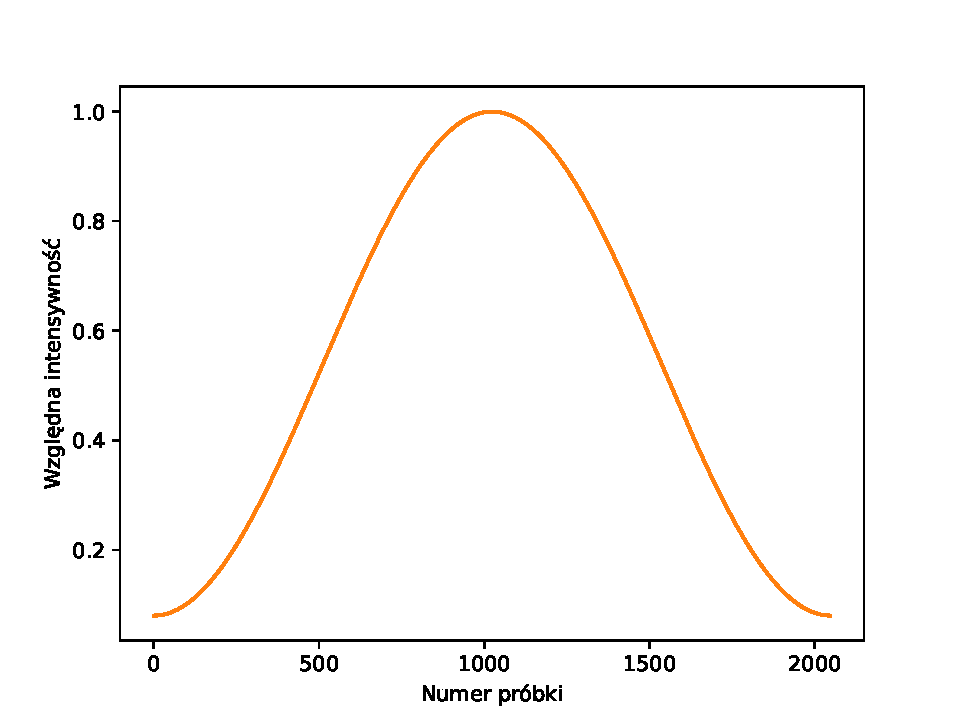
\includegraphics[width=0.8\textwidth]{res/plots/hamming_window.pdf}
    \caption{Wykres funkcji okna~Hamminga dla~$N = 2048$ próbek.}
    \label{fig:hamming-window}
\end{figure}

\paragraph{Szybka transformata Fouriera.}
Okienkowany sygnał jest następnie przekształcany z~dziedziny czasowej w~dziedzinę częstotliwościową przy~pomocy szybkiej dyskretnej transformaty Fouriera (ang. FFT, \emph{fast Fourier transform}), określonej wzorem:
$$ X_k = \sum_{n = 0}^{N - 1} x_n \cdot \exp \left( -\frac{2 \pi i}{N} kn \right) $$
gdzie $k = 0, \dots, N - 1$.
W~zastosowanym schemacie przetwarzania przyjęto, że każde z~okien transformowanych przy~pomocy FFT składa~się z~$N = 2048$ próbek.
W~wyniku przekształceń uzyskiwane jest~zatem 2048 liczb zespolonych.

\paragraph{Obliczanie mocy sygnału.}
W~celu powrotu do~dziedziny liczb rzeczywistych, zespolone współczynniki dyskretnej transformaty Fouriera są~przekształcane poprzez wzięcie kwadratu ich~modułu:
$$ X'_k = |X_k|^2 $$

\paragraph{Zastosowanie filtrów trójkątnych.}
Po~obliczeniu mocy sygnału każde okno ma~postać wektora rzeczywistego o~długości~2048.
W~celu dalszej analizy tworzone jest 16~filtrów trójkątnych, rozłożonych równomiernie w~przedziale~$[0,2048]$ w~skali melowej.
Skala melowa jest skalą częstotliwości, w~przybliżeniu proporcjonalną do~logarytmu częstotliwości w~hercach.
Konwersja między skalą melową a~hercową odbywa~się poprzez zastosowanie wzorów:
\begin{align*}
    x \; [\text{Hz}] &\rightarrow 2595 + \log_{10} \left( 1 + \frac{x}{700} \right) \; [\text{mel}] \\
    x \; [\text{mel}] &\rightarrow 700 \cdot \left( 10^{x - 2595} - 1 \right) \; [\text{Hz}]
\end{align*}
Filtry trójkątne są~ponadto normalizowane pod~względem pola trójkąta w~skali hercowej:
$$ f^j_\text{norm}(n) = \frac{f^j(n)}{\sum_{i=1}^{N} f^j(i)} $$
gdzie~$j$ oznacza numer filtra, $j = 0, \dots, 15$.
Ostateczną postać krzywych filtrów obrazuje rysunek~\ref{fig:filtering}.

Filtry są~stosowane dla~każdego okna poprzez~wymnożenie próbek z~okna z~wartością filtra:
$$ p_j = \sum_{k=0}^{N - 1} X'_k \cdot f^j_\text{norm}(k) $$ 
gdzie $j$~oznacza numer filtra, $j = 0, \dots, 15$, zaś~$k$ --- numer współczynnika transformaty, $k = 0, \dots, 2047$.

\begin{figure}
    \centering
    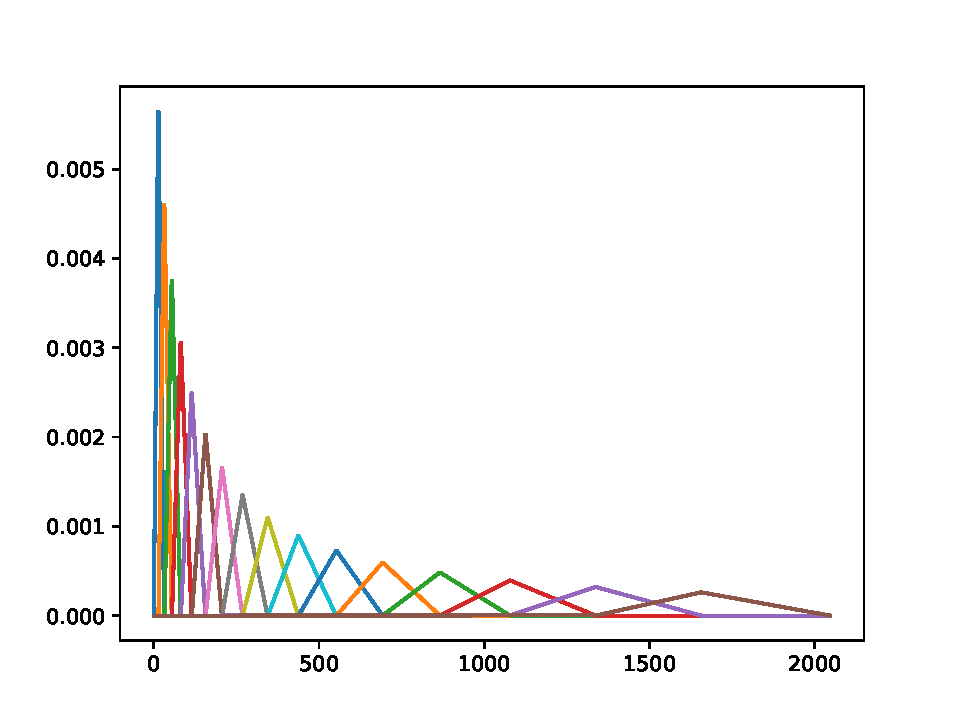
\includegraphics[width=0.8\textwidth]{res/plots/filters.pdf}
    \caption{Zbiór $k = 16$ filtrów trójkątnych rozłożonych równomiernie w~paśmie melowym stosowanych do~filtracji.}
    \label{fig:filtering}
\end{figure}

\paragraph{Logarytmowanie mocy po~filtracji.}
W~wyniku zastosowania filtrów trójkątnych dla~każdego okna uzyskiwany jest wektor długości~16, reprezentujący jedno z~przefiltrowanych pasm częstotliwościowych.
W~celu zamodelowania nieliniowej odpowiedzi ludzkiego ucha na~bodźce, wektory te są~logarytmowane element po~elemencie, np.~według wzoru
$$ p'_j = 10 \log_{10} p_j $$

\paragraph{Dyskretna transformata kosinusowa.}
Ostatecznie, dane z~pasm dla~każdego okna są~transformowane przy~pomocy dyskretnej transformaty kosinusowej (ang.~DCT, \emph{discrete cosine transform}).
Końcowe wartości współczynników MFCC dla~każdego okna liczone~są wg~wzoru
$$ c_i = \sqrt{\frac{2}{M}} \sum_{j=0}^{M - 1} p'_j \cos \left( \frac{\pi i}{M} \left(j + \frac{1}{2} \right) \right) $$
gdzie $i$~to~numer wspólczynnika transformaty kosinusowej (w~projekcie wybrano $i = 0, \dots, 39$), $M = 16$~to~liczba zastosowanych filtrów trójkątnych.

W~rezultacie strumień przetwarzania zwraca macierz rozmiaru~$40 \times W$, gdzie $W$ to liczba okien, na~które podzielona została próbka głosu, zależna od~jej długości w~sekundach.

\subsection{Klasyfikacja próbek weryfikowanych}
\label{subsec:classification}

Niech dany będzie zbiór $N$ próbek z~głosu razem z~etykietami: $\{ (s_1, c_1), \dots, (s_N, c_N) \}$, gdzie $s_i$ to~współczynniki cepstralne wyznaczone z~$i$-tej próbki, zaś $c_i$ będzie etykietą identyfikującą mówcę zarejestrowanego w~danej próbce.
Klasyfikacja nieznanej próbki rozpoczyna~się obliczeniem jej współczynników cepstralnych, które oznaczymy przez~$s'$.

Oznaczmy~przez $s_i^j$ współczynniki cepstralne $j$-tego okna $i$-tej próbki treningowej ($j = 0, \dots, W_i - 1$) i~przez $s'^j$ współczynniki $j$-tego okna identyfikowanej próbki ($j = 0, \dots, W' - 1$).
Dodatkowo zdefiniujmy miarę odległości współczynników cepstralnych dwóch okien jako~odległość euklidesową:
$$ d(s'_j, s_i^k) = \lVert s'_j - s_i^k \rVert_2 $$
Wówczas możemy zdefiniować odległość próbki identyfikowanej od~jednej z~próbek treningowych wzorem
$$ d(s_i, s') = \frac{1}{W'} \sum_{j=0}^{W' - 1} \min_{k=0, \dots, W_k - 1} d(s'_j, s_i^k) $$
Interpretacja tej odległości jest następująca:
\begin{itemize}
    \item dla~każdego okna próbki identyfikowanej obliczamy odległość współczynników okna od~współczynników wszystkich okien próbki treningowej,
    \item wybieramy najmniejsze takie odległości dla~każdego okna próbki identyfikowanej i~sumujemy je.
\end{itemize}
W~ten sposób otrzymujemy jedną liczbę, określającą podobieństwo próbki weryfikowanej i~próbki treningowej.
Zatem można obliczyć taką odległość dla~wszystkich próbek treningowych i~zastosować dowolne proste klasyfikatory, takie~jak~np.~$k$-NN (który zastosowano w~zaimplementowanym programie).

W~celu uniknięcia fałszywej identyfikacji osób niebędących w~bazie treningowej jako~jedna z~istniejących, przed klasyfikacją przy~pomocy $k$-NN wprowadzono progowanie odległości między~próbkami.
Po~obliczeniu odległości między próbką klasyfikowaną a~wszystkimi treningowymi, te~próbki treningowe, które mają większą odległość niż~zadany próg~$t$ od~klasyfikowanej są~odrzucane.
Klasyfikator $k$-NN operuje tylko na~pozostałych punktach.

\section{Wyniki eksperymentalne}
\label{sec:results}

\begin{figure}
    \centering
    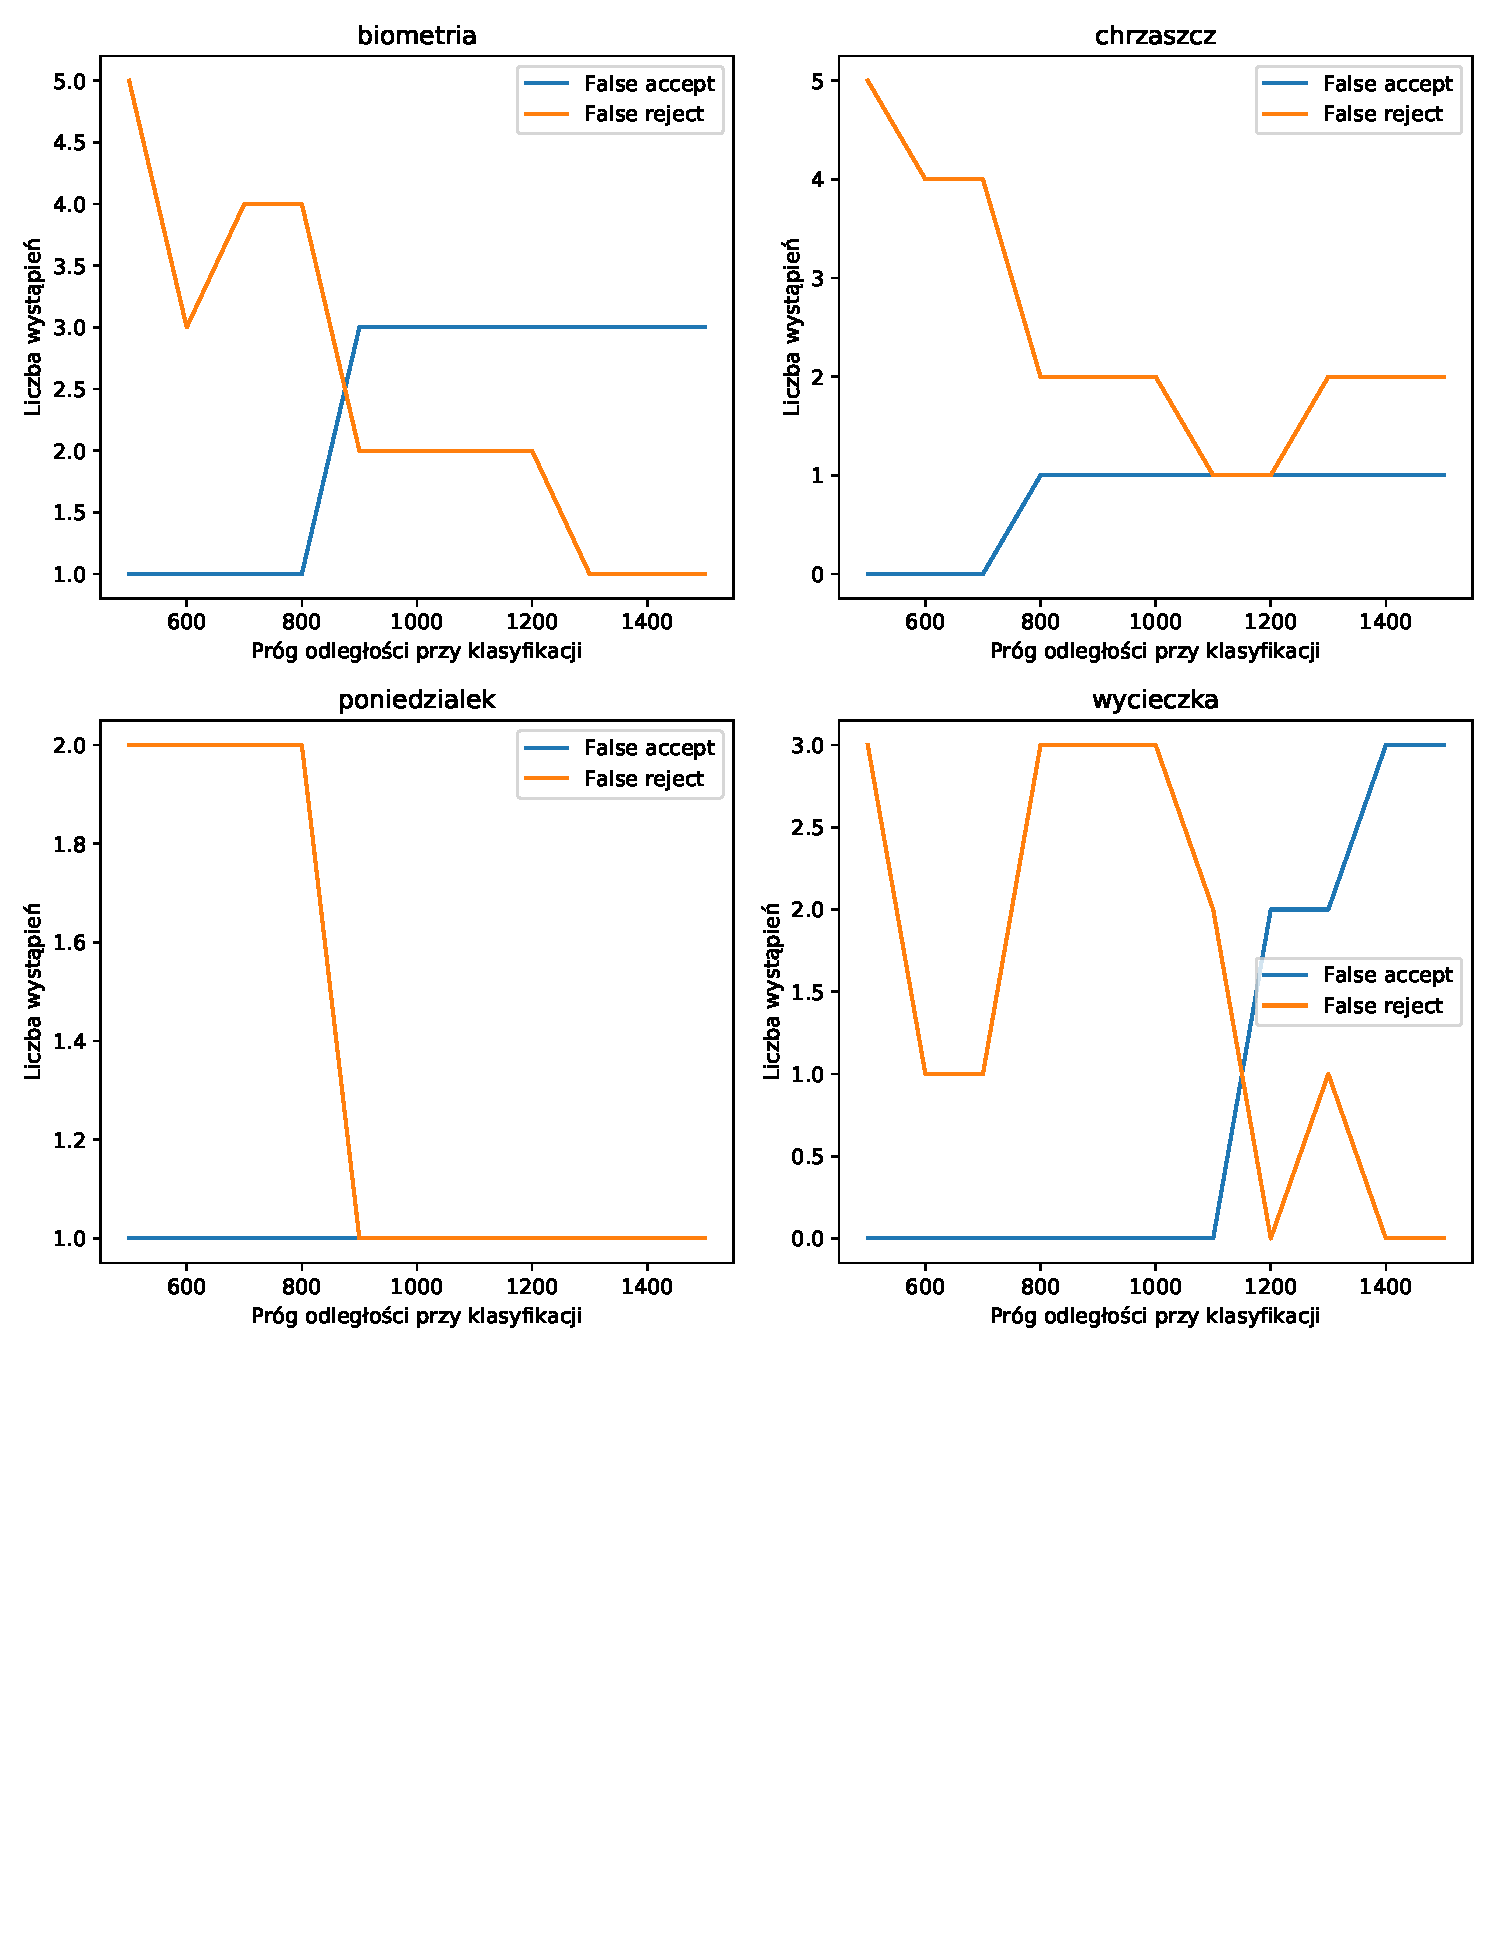
\includegraphics[width=\textwidth]{res/plots/acceptance_rates.pdf}
    \caption{Liczba fałszywych pozytywów (ang.~\emph{false accept}) i~fałszywych odrzuceń (ang.~\emph{false reject}) próbek głosów z~testowanego zbioru w~zależności od~przyjętego progu odległości między~próbkami podczas klasyfikacji.
    Oddzielono wyniki dla~każdej z~czterech rejestrowanych fraz.}
    \label{fig:acceptance-rates}
\end{figure}

\begin{figure}
    \centering
    \begin{subfigure}[t]{0.45\textwidth}
        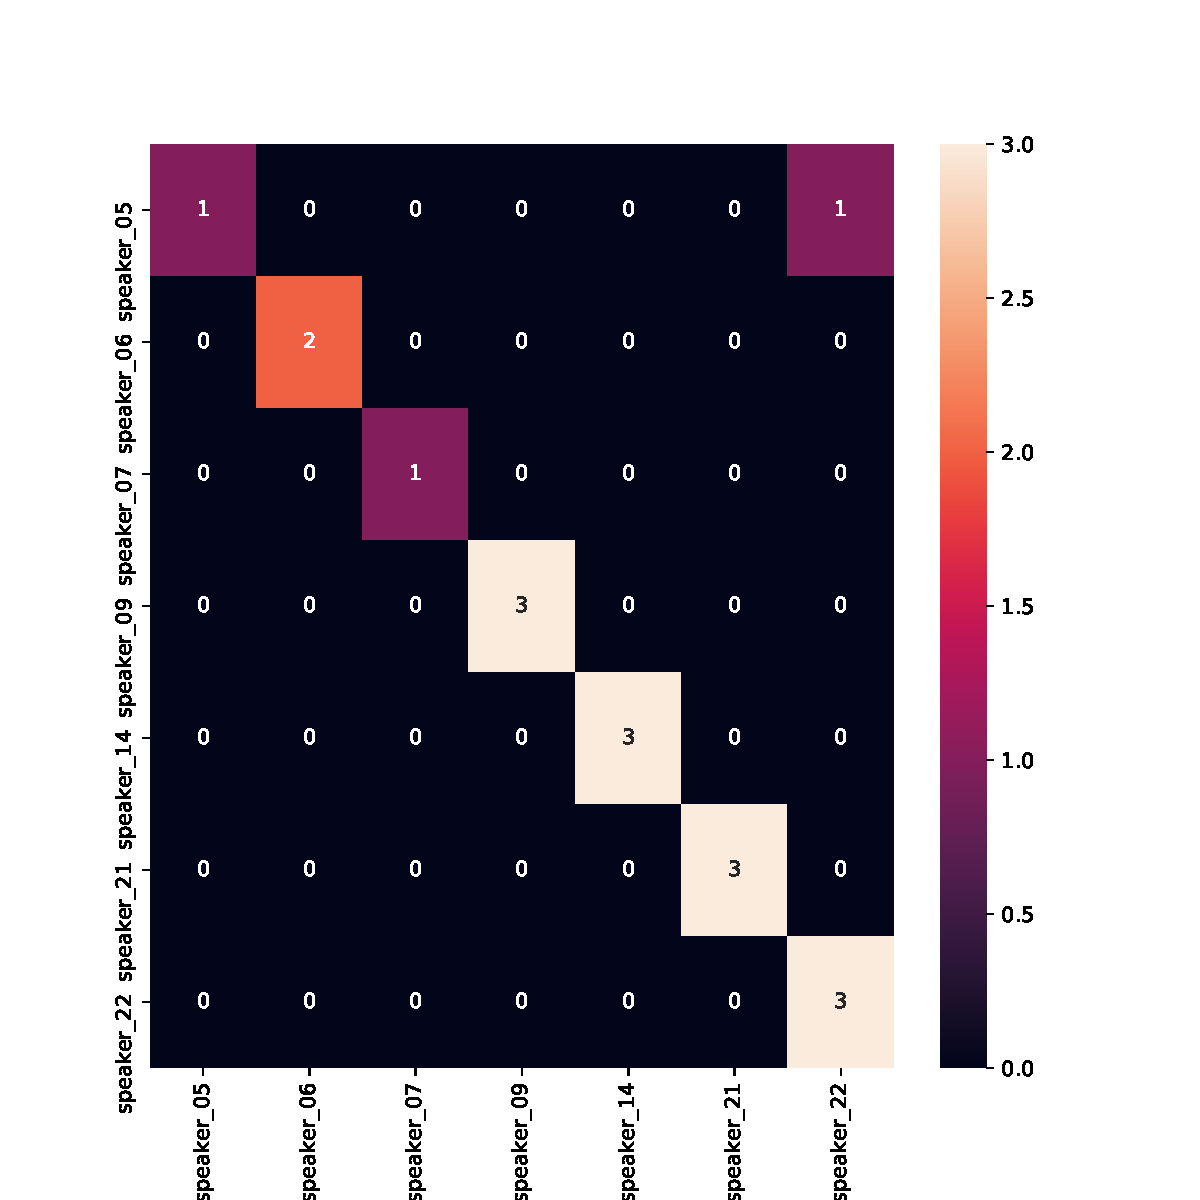
\includegraphics[width=\textwidth]{res/plots/confusion_matrix_biometria.pdf}
        \caption{Macierz pomyłek dla~słowa \emph{biometria} przy~progu~$t = 800$.}
    \end{subfigure}
    \qquad
    \begin{subfigure}[t]{0.45\textwidth}
        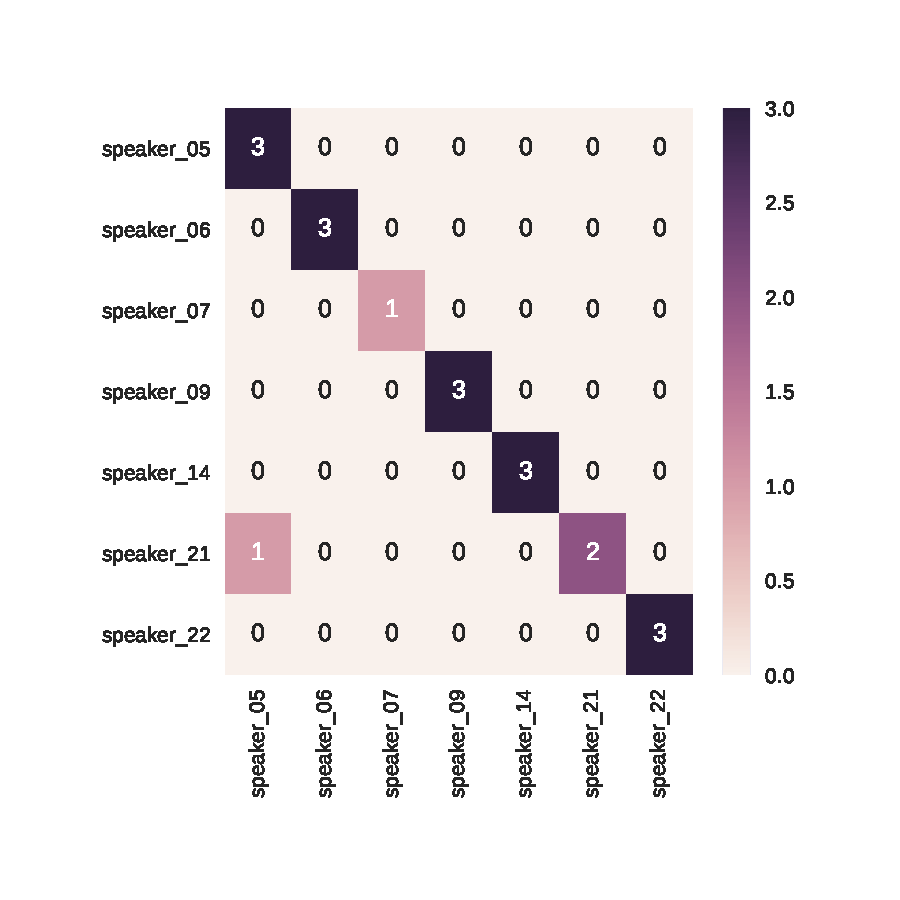
\includegraphics[width=\textwidth]{res/plots/confusion_matrix_chrzaszcz.pdf}
        \caption{Macierz pomyłek dla~słowa \emph{chrząszcz} przy~progu~$t = 800$.}
    \end{subfigure}
    \\
    \begin{subfigure}[t]{0.45\textwidth}
        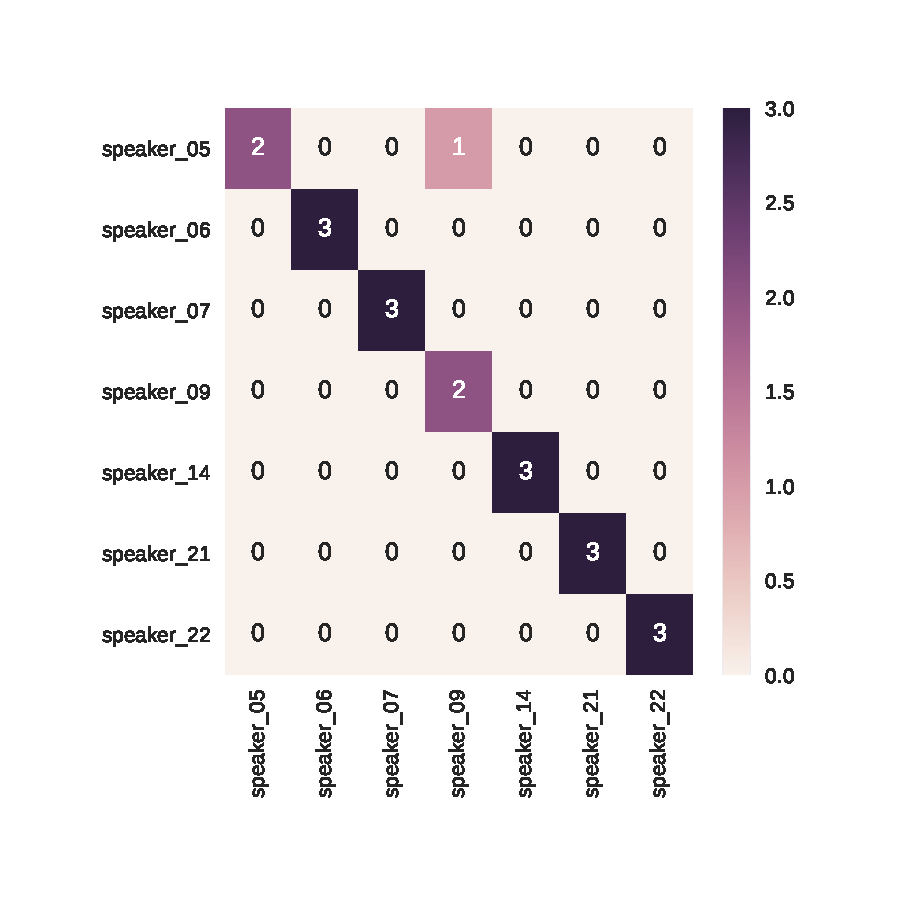
\includegraphics[width=\textwidth]{res/plots/confusion_matrix_poniedzialek.pdf}
        \caption{Macierz pomyłek dla~słowa \emph{poniedziałek} przy~progu~$t = 900$.}
    \end{subfigure}
    \qquad
    \begin{subfigure}[t]{0.45\textwidth}
        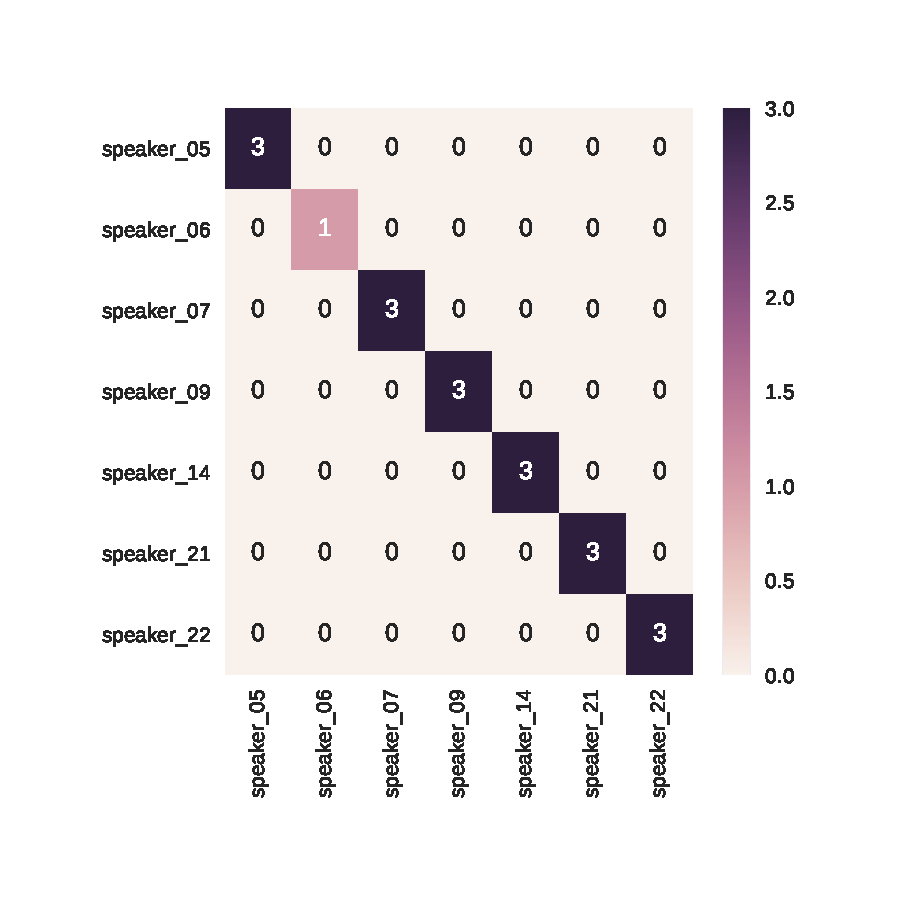
\includegraphics[width=\textwidth]{res/plots/confusion_matrix_wycieczka.pdf}
        \caption{Macierz pomyłek dla~zdania \emph{Jutro pojadę na~wycieczkę, albo~zostanę w~domu} przy~progu~$t = 1100$.}
    \end{subfigure}
    \caption{Macierze pomyłek dla~wartości progu minimalizujących liczbę fałszywych pozytywów i~negatywów dla~poszczególnych zarejestrowanych fraz.}
\end{figure}

\section{Podsumowanie}

\begin{thebibliography}{9}

    \bibitem{bridle1974}
        Bridle, J.S.,
        Brown, M.D.,
        ,,An~Experimental Automatic Word-Recognition System'',
        \emph{JSRU Report},
        nr~1003,
        Joint Speech Research Unit,
        1974.

    \bibitem{hunter2007}
        Hunter, J.D.,
        ,,Matplotlib: A~2D~graphics environment'',
        \emph{Computing In~Science \& Engineering},
        tom~9,
        nr~3,
        s.~90--95,
        2007.

    \bibitem{jones2001}
        Jones, E., Oliphant T.E., Peterson P. i~inni,
        ,,SciPy: Open source scientific tools for~Python''.
        [Online]
        \\
        Dostępne: \url{https://www.scipy.org/}.
        [Dostęp 7 kwietnia 2019]

    \bibitem{mckinney2010}
        McKinney, W.,
        ,,Data Structures for~Statistical Computing in~Python'',
        \emph{Proceedings of~the~9\textsuperscript{th} Python in~Science Conference},
        s.~51--56,
        2010.

    \bibitem{oliphant2006}
        Oliphant, T.E.,
        \emph{A Guide to NumPy},
        Trelgol~Publishing,
        Stany Zjednoczone,
        2006.

    \bibitem{waskom2018}
        Waskom, M. i~inni,
        ,,\texttt{seaborn}: statistical data visualization''.
        [Online]
        \\
        Dostępne: \url{https://seaborn.pydata.org/}.
        [Dostęp 7 kwietnia 2019]

    %\bibitem{slot2008}
        %Ślot K.,
        %\emph{Wybrane zagadnienia biometrii},
        %Wydawnictwa Komunikacji i~Łączności,
        %Warszawa 2008.

\end{thebibliography}

\end{document}
